%% LyX 2.0.2 created this file.  For more info, see http://www.lyx.org/.
%% Do not edit unless you really know what you are doing.
\documentclass[12pt,a4paper,slovak,czech,notitlepage]{report}
\usepackage{lmodern}
\usepackage[T1]{fontenc}
\usepackage[utf8]{inputenc}
\usepackage{listings}
\setcounter{secnumdepth}{3}
\setcounter{tocdepth}{3}
\usepackage{color}
\usepackage{babel}
\usepackage{varioref}
\usepackage{rotfloat}
\usepackage{textcomp}
\usepackage{url}
\usepackage{graphicx}
\usepackage{nomencl}
% the following is useful when we have the old nomencl.sty package
\providecommand{\printnomenclature}{\printglossary}
\providecommand{\makenomenclature}{\makeglossary}
\makenomenclature
\usepackage[unicode=true,
 bookmarks=true,bookmarksnumbered=false,bookmarksopen=true,bookmarksopenlevel=1,
 breaklinks=false,pdfborder={0 0 0},backref=false,colorlinks=true]
 {hyperref}
\hypersetup{pdftitle={Bakalářská práce},
 pdfauthor={Jakub Kinšt},
 pdfsubject={Systém pro podporu výuky}}
\usepackage{breakurl}

\makeatletter

%%%%%%%%%%%%%%%%%%%%%%%%%%%%%% LyX specific LaTeX commands.
\special{papersize=\the\paperwidth,\the\paperheight}

%% A simple dot to overcome graphicx limitations
\newcommand{\lyxdot}{.}


%%%%%%%%%%%%%%%%%%%%%%%%%%%%%% User specified LaTeX commands.
\usepackage{a4wide}
\usepackage[left=4cm]{geometry}

\renewcommand\nomname{Seznam použitých zkratek}

\makeatother

\begin{document}
\pagestyle{empty}

\selectlanguage{slovak}%
\begin{center}
\vspace{15mm}

\par\end{center}

\begin{center}
{\large Univerzita Karlova v Praze}\\
{\large Matematicko-fyzikální fakulta\vspace{5mm}
}
\par\end{center}{\large \par}

\begin{center}
\textbf{\Large BAKALÁŘSKÁ PRÁCE\vspace{10mm}
}
\par\end{center}{\Large \par}

\begin{center}
\includegraphics[scale=0.3]{logo}
\par\end{center}

\selectlanguage{czech}%
\begin{center}
{\Large \vspace{15mm}
Jakub Kinšt \vspace{5mm}
}
\par\end{center}{\Large \par}

\begin{center}
\textbf{\Large Systém pro podporu výuky\vspace{5mm}
}
\par\end{center}{\Large \par}

\begin{center}
\textbf{\large Ústav formální a aplikované lingvistiky, MFF UK\vspace{15mm}
}
\par\end{center}{\large \par}

\noindent \begin{center}
{\large Vedoucí bakalářské práce: Mgr. Miroslav Týnovský \vspace{2mm}
}
\par\end{center}{\large \par}

\noindent \begin{center}
{\large Studijní program: Informatika\vspace{2mm}
}
\par\end{center}{\large \par}

\noindent \begin{center}
{\large Studijní obor: Obecná Informatika\vspace{20mm}
}
\par\end{center}{\large \par}

\begin{center}
{\large Praha 2012}
\par\end{center}{\large \par}

\noindent \newpage{}TODO: Zde bude poděkování

\noindent \newpage{}\vspace*{\fill}
\noindent

\noindent Prohlašuji, že jsem tuto bakalářskou práci vypracoval samostatně
a výhradně s použitím citovaných pramenů, literatury a dalších odborných
zdrojů. 

\vspace{10mm}


\noindent \noindent

\noindent Beru na vědomí, že se na moji práci vztahují práva a povinnosti
vyplývající ze zákona č. 121/2000 Sb., autorského zákona v platném
znění, zejména skutečnost, že Univerzita Karlova v Praze má právo
na uzavření licenční smlouvy o užití této práce jako školního díla
podle § 60 odst. 1 autorského zákona.\bigskip{}


\noindent V Praze dne \hfill{}podpis

\newpage{}

\noindent \noindent

\noindent Název práce: Systém pro podporu výuky\\
Autor: Jakub Kinšt\\
Katedra (ústav): Ústav formální a aplikované lingvistiky\\
Vedoucí bakalářské práce: Mgr. Miroslav Týnovský \\
e-mail vedoucího: tynovsky@ufal.mff.cuni.cz\\


\noindent Abstrakt: V předložené práci je implementována webová služba
usnadňující práci lektorům i studentům libovolného prezenčního kurzu.
Umožní jednoduchou, ale účinnou komunikaci mezi lektorem a studenty
i mezi studenty navzájem pomocí komentářů, soukromých zpráv, nebo
diskuzního fóra. Poskytne možnost publikovat průběžné výsledky studentů,
umožní studenty vyzkoušet z probrané látky pomocí online testů, oznámit
studentům jakékoliv blížící se termíny a další. Součástí práce je
i implementace nativní aplikace pro platformu Google Android, která
zpřístupní většinu funkcí služby z pohodlí mobilního zařízení. Rozhraní
pro propojení s mobilní aplikací je oddělené a univerzálně použitelné
pro již existující webovou aplikaci. Prakticky bez zásahu do stávajícího
zdrojového kódu lze aplikaci propojit s klientem v mobilním zařízení
během několika málo minut.\\


\noindent Klíčová slova: XXX

\vspace{10mm}


\noindent \noindent

\noindent Title: Learning management system\\
Author: Jakub Kinšt\\
Department: Institute of Formal and Applied Linguistics\\
Supervisor: Mgr. Miroslav Týnovský

\noindent Supervisor's e-mail address: tynovsky@ufal.mff.cuni.cz\\


\noindent Abstract: Presented thesis implements web service helping
lectors and students of an arbitrary full-time course. It provides
simple, but effective communication between lector and students or
between students each other via comments, private message system,
or via forum. It offers possibility to publish student's results,
to test students via online assignments and to provide information
about arbitrary upcoming events. The thesis includes implementation
of native application for Google Android platform bringing most of
the features directly to user's mobile device. The interface between
the web application and the mobile application is developed separately
and it is universally applicable to an existing web application implementation.
Thanks to this interface, it is possible to connect to a mobile application
in matter of minutes and practically without affecting any of the
existing source code.\\


\noindent Keywords: XXX \newpage{}

\pagestyle{headings}\setcounter{page}{1}\tableofcontents{}

\newpage{}


\chapter{Úvod}


\section{Motivace}

Profesoři, učitelé, cvičící a lektoři kurzů se často potýkají s problémem,
jak své studenty spolehlivě informovat o průběhu výuky, jak jim poskytnout
studijní materiál a jiné doplňující informace. Rádi by také čas od
času studenty rychle a hlavně jednoduše vyzkoušeli z probrané látky.
Studenti chtějí mít k dispozici způsob, jakým mohou lektorovi nebo
samotnému učiteli položit otázku a případně na dané téma diskutovat.
Chtějí také dostávat aktuální informace o blížících se termínech nebo
testech.

Řešením je pro některé lektory rozesílání aktuálních informací pomocí
hromadných e-mailů, které jsou nepraktické a v poštovní schránce rychle
upadnou v zapomnění. Pokud vznese student dotaz, dostane se odpovědi
jen jemu a ostatní se o ní většinou vůbec nedozvědí.

Iniciativnější lektoři s nemalou trochou úsilí vytvoří jednoduchý
web, který se snaží pravidelně aktualizovat a přidávat novinky. Často
ale stejně chybí možnost diskuze, nahrávání materiálů, správa událostí
a online vypracování testů a úkolů. Přestože lze některé z těchto
vlastností nahradit externími webovými službami, bylo by dobré mít
po ruce komplexní a zároveň uživatelsky jednoduché řešení, které všechny
zmíněné problémy vyřeší.

Zároveň, v době chytrých mobilních telefonů a pohodlnosti mobilního
internetu, by se hodilo, aby měl uživatel veškerý obsah na dosah i
ve svém mobilním telefonu (nebo v jiném mobilním zařízení), a mohl
si tak číst aktuality na cestách nebo vyplňovat test po cestě do školy
ve vlaku.

Výsledkem práce je implementace kompletního univerzálního řešení webové
služby zajišťující podporu pro standardní prezenční výuku. Služba
ulehčí práci jak lektorům, tak i studentům libovolného kurzu. Umožní
lektorovi jednoduše kontaktovat všechny studenty, informovat je o
průběhu a obsahu jednotlivých lekcí/přednášek/cvičení, oznámit dosavadní
výsledky studentům, poskytnout jim libovolné elektronické učební materiály
ke stažení, zadat jim elektronický test nebo úkol s různými typy otázek
a informovat je o nadcházejících událostech či termínech. Studenti
mohou diskutovat pod jednotlivými lekcemi/přednáškami/cvičeními, diskutovat
v diskuzním fóru na jakékoliv relevantní téma jak s ostatními studenty,
tak i se samotným lektorem/lektory a mohou si mezi sebou posílat soukromé
zprávy.

Většinu z těchto aktivit je také možné provozovat skrze nativní aplikaci
pro mobilní platformu Google Android\cite{android} z pohodlí mobilního
telefonu nebo jiného mobilního zařízení (z tabletu, přehrávače apod.).

Součástí práce je také samostatná implementace univerzálního řešení
propojení webové aplikace (postavené na Nette Frameworku\cite{nette})
s mobilní aplikací pro platformu Google Android.

Výhodou je nezávislost na konkrétní vzdělávací instituci (škola, univerzita,
apod.) a také to, že aplikace bude nabízena jako služba (ne software),
tudíž se uživatel vyhne jakékoliv instalaci, složité konfiguraci a
náročnému provozu a správě výukového systému. V případě rozšíření
aplikace má navíc jak student, tak i lektor všechny studované (resp.
vyučované) kurzy k dispozici pohromadě, na jednom místě a stejně (přiměřeně)
jednoduše ovladatelné.


\section{Struktura práce}

TODO: zkontrolovat nakonec cislovani kapitol

V následující kapitole (Kapitola 2) jsou shrnuty dosavadní existující
implementace podobného, nebo stejného typu aplikace, jejich klady
a zápory. Ve třetí kapitole je popsána architektura objektového programování
MVC\nomenclature{MVC}{Model-View-Controller} (Model-View-Controller),
kterou se implementovaná aplikace řídí. Ve čtvrté kapitole je teoreticky
rozebrána problematika propojení webové aplikace s aplikací pro mobilní
zařízení, zejména takzvané ,,otevření API%
\footnote{Application Programming Interface%
}\nomenclature{API}{Application Programming Interface}'' webové aplikace.
V další části jsou popsány a vysvětleny zajímavé technologie a frameworky,
které byly při implementaci použity. Následně jsou vysvětleny postupy
při implementaci práce - nejdříve webové aplikace, potom propojení
s mobilní aplikací a nakonec samotné mobilní aplikace pro platformu
Android. V desáté kapitole je sepsaná uživatelská dokumentace k aplikaci,
minimální požadavky a pokyny k instalaci. Na konci práce je k dispozici
seznam příloh a vysvětleny všechny použité zkratky.


\chapter{Existující implementace}

Implementovaná aplikace z velké části spadá do skupiny systémů pro
správu výuky (\emph{LMS}%
\footnote{\emph{Learning Management System}%
}\nomenclature{LMS}{Learning Management System}). Při výběru systému
není k dispozici příliš mnoho možností. Existuje několik komerčních
řešení kompletní správy výuky včetně e-learningu (výuka na dálku),
které mohou být ,,ušity'' na míru klientovi a dále několik otevřených
(open-source) řešení, do kterých je ze strany uživatele potřeba vložit
nemalé úsilí (ať už do instalace, do úprav podle vlastních potřeb,
nebo samotného provozování aplikace).


\section{Moodle}

Moodle\cite{moodle} (Modular Object-Oriented Dynamic Learning Environment)\emph{
}je jedno z open-source webových řešení systému pro správu výuky.
Jako většina řešení LMS se Moodle zaměřuje převážně na podporu či
kompletní řešení dálkové výuky (e-learning). Přesto ho mnoho uživatelů
využívá i k podpoře klasické prezenční výuky. Moodle je nabízen jako
open-source software (ne jako služba) - to znamená, že je třeba jej
odborně nainstalovat na vlastní server, nakonfigurovat podle vlastních
potřeb a hlavně provozovat, protože mnoho operací je závislých na
existenci stálého administrátora. Výhodou je relativně jednoduchá
rozšiřitelnost. Se znalostí programování v PHP%
\footnote{Hypertext Preprocessor%
}\nomenclature{PHP}{Hypertext Preprocessor}\cite{php} lze systém
rozšířit o další moduly, které mohou implementovat konkrétní požadavky
,,ušité'' na míru. Tento systém používá mnoho světových univerzit,
škol a jiných výukových institucí. Jelikož si provoz musí řešit každá
instituce sama, neexistuje žádné univerzální místo, kde by měl uživatel
dostupné kurzy nezávisle na škole, nebo univerzitě. Nevýhody tkví
v náročnosti na provoz a údržbu aplikace a dále nepříliš intuitivní
a místy složité ovládání aplikace. Rozhraní se podobá (i ze strany
studenta) spíše složitému informačnímu systému a typická podstránka
obsahuje nadmíru možností a uživatelských voleb. Potíže nastávají,
pokud uživatel potřebuje založit kurz netýkající se konkrétní instituce.
Pokud si sám nezprovozní vlastní instanci systému, nezbývá mu mnoho
možností. Systém je implementován v programovacím jazyce PHP.

Některé ze zmíněných nevýhod lze eliminovat využitím služeb serveru
\emph{moodlerooms.com}, který za poplatek nabízí hostování a správu
systému Moodle včetně ukládání dat do cloudu (na servery \emph{moodlerooms.com}).
V praxi se pak dá říci, že systém je nabízen jako služba.

Co se týče propojení s aplikací pro mobilní zařízení, zatím neexistuje
žádné oficiální řešení. Je k dispozici pouze několik málo neoficiálních
aplikací, které však implementují jen zlomek základních modulů systému.
Za zmínku stojí pouze aplikace mTouch\cite{mtouch} pro platformu
iOS, která se řadí mezi ty zdařilejší.


\section{Blackboard}

Blackboard\cite{blackboard} je komerční software určený pro kompletní
správu výuky velkých institucí - převážně univerzit v USA. Toto řešení
většinou není dostupné jednotlivcům nebo menším organizacím. Má mnoho
společných rysů se systémem Moodle, z čehož plynou i společné nevýhody.
Opět je hlavním účelem podpora vzdáleného (neprezenčního) vyučování
- nabízí virtuální vyučování a podobně. Výhodou je ale podpora ze
strany autorské společnosti (prodejce). Společnost za poplatky nabízí
instalaci, hostování aplikace i správu a zajištění provozu.

Autoři nabízejí nativní aplikaci pro většinu platforem mobilních zařízení,
která však podle dostupných uživatelských zkušeností zdaleka není
kompatibilní se všemi konkrétními instancemi běžících na univerzitách.


\section{Instructure Canvas}

Třetí implementací stojící za zmínění je systém Instructure Canvas\cite{instructure-canvas}.
Původně šlo o komerční produkt, ale v únoru 2011 se z aplikace stala
open-source platforma. Canvas se snaží ,,ukrojit'' část úspěchu
systému Moodle a díky podobným vlastnostem a funkcím s výrazně modernějším
pojetím se mu to daří. Aplikace si zakládá na moderním designu a přiměřené
uživatelské jednoduchosti - využívá novodobé technologie jako HTML5%
\footnote{HyperText Markup Language%
}\nomenclature{HTML}{HyperText Markup Language}, CSS3\emph{}%
\footnote{\emph{Cascading Style Sheets}%
}\emph{\nomenclature{CSS}{Cascading Style Sheets}} či jQuery a dokáže
částečně spolupracovat s oblíbenými sociálními službami. Velikou výhodou
je to, že aplikace je provozována i jako služba. Tudíž uživateli odpadají
starosti se složitou instalací, konfigurací, aktualizacemi a samotným
provozem aplikace. Zároveň jsou všechna data spolehlivě uložena v
cloudu (na serverech společnosti Instructure). Podobnost s platformou
Moodle však opět přináší nevýhody vycházející z vysoké orientace na
e-learning a minimálního zaměření na podporu prezenční výuky. Aplikace
je implementována především v jazyce Java a webová služba funguje
díky technologii Google AppEngine.

Společnost Instructure nabízí oficiální mobilní aplikaci, avšak pouze
pro platformu iOS. Pro Android neexistuje zatím žádné (ani neoficiální)
řešení.


\chapter{Architektura MVC}

Architektura MVC\emph{}%
\footnote{\emph{Model-View-Controller}%
}\emph{\cite{mvc}} se poslední dobou stává standardem při vývoji objektově
orientovaných (nejen) webových aplikací. Přináší totiž mnohé výhody,
klady a usnadnění.

Architektura byla poprvé definována již v sedmdesátých letech minulého
století společností Smalltalk.\emph{ }Rozděluje implementaci objektově
orientované aplikace do tří základních vrstev: Model (Vrstva modelu),
View (Vrstva pohledu), Controller (Vrstva řadiče). Vrstvy v zásadě
izolují ty součásti implementace, které spolu souvisí, musí o sobě
navzájem vědět konkrétní charakteristiky a často je lze chápat samostatně.

Model je vrstva, která obvykle obstarává nebo udržuje informace a
implementuje nějaký obecný problém nezávisle na získávání vstupních
dat nebo prezentování výsledků. Obvykle se jedná o jednu, nebo několik
tříd, které například získávají data z databázové vrstvy, provádí
výpočty a jiné podobné úkony. Model by na ostatních vrstvách neměl
být vůbec závislý.

View (Pohled), jak název napovídá, je vrstva, která má za úkol zobrazovat
výsledná data. Zobrazovat je nemusí jen uživateli, ale například také
jinému programu (zobrazuje API), tudíž se nemusí vždy jednat o grafické
rozhraní. Zpravidla je však pohled reprezentován právě definicí uživatelského
rozhraní - HTML šablony, GUI%
\footnote{Graphical User Interface%
}\nomenclature{GUI}{Graphical User Interface} aplikace.

Controller (Řadič) je vrstva, o které lze říci, že leží mezi vrstvami
Model a View. Stará se převážně o zpracování uživatelského vstupu
a o propojení modelu s pohledem. Obvykle získává parametry ze vstupu,
ty předá modelu, který na jejich základě vrátí potřebná data nebo
učiní jiné úkony. Případná získaná data zase předá pohledu, který
je vhodným způsobem podá například uživateli.

Výhod následování pravidel MVC je mnoho. Tou hlavní je nepochybně
obrovská přehlednost výsledného kódu. Ta je způsobena striktním oddělením
uživatelského rozhraní (View) od kódu obsluhy (Controller) a aplikační
logiky (Model). Díky tomu jsou také aplikace daleko lépe připravené
na případné úpravy či rozšíření - například změna vzhledu uživatelského
rozhraní proběhne pouze na úrovni vrstvy View, tedy vyvíjet lze takřka
odděleně. Výhodou je také to, že při testování aplikace je možné testovat
jednotlivé vrstvy implementace naprosto odděleně.


\chapter{Problematika propojení s mobilní aplikací}


\section{Motivace}

V posledních letech je viditelný významný přesun práce s internetem
z domácích počítačů na mobilní zařízení. Mobilními zařízeními jsou
myšleny především mobilní telefony a tablety. Provozovatelé webových
služeb jsou tak stále častěji nuceni umožnit klientovi pohodlně a
naplno užívat aplikaci právě z těchto zařízení.

Někteří tento trend řeší cestou (obvykle) nejmenšího odporu - optimalizací
webových stránek aplikace pro menší obrazovky přenosných zařízení.
Toto řešení spolu ale často nese několik značných nevýhod. Aplikace
především nemůže naplno využít potenciál zařízení. Neposkytují takový
komfort jako aplikace integrované do systému (například pro zobrazování
oznámení), které mohou využívat kompletní sadu frameworků dodávaných
výrobcem operačního systému. Nelze aplikaci integrovat do systému
nebo například přistupovat k datům z jiných aplikací, jako je seznam
kontaktů, kalendář a jiné. Nedokáží ani naplno využívat některé hardwarové
technologie zabudované v moderních zařízeních, jako jsou senzory polohy,
světla, zrychlení, fotoaparát a podobně, které mohou být často užitečné.

Toto řešení také kompletně znepřístupní obsah v případě nedostupnosti
internetového připojení. Uživatel tedy může aplikaci používat pouze
pokud je v tu chvíli připojen k internetu.

Jistou nadějí pro tento přístup může být technologie webových stránek
v HTML5\cite{html5}. Ta přidává do tradičních HTML stránek možnost
využít některé z těchto pokročilých funkcí. Je zde možnost obsah ke
klientovi uložit a pak ho zobrazit offline - tedy krátkodobě bez připojení
k internetu. Pomocí HTML5 elementů je také možné zjistit polohu uživatele
pomocí zabudovaných senzorů. Další novinkou je element\emph{ }\inputencoding{latin2}\lstinline!<canvas>!\inputencoding{utf8},
který umožňuje do okna prohlížeče vykreslovat libovolnou grafiku.
HTML v této verzi již také nativně podporuje přehrávání videa nebo
audia - už není nutné vytvářet proprietární přehrávače například pomocí
technologie Flash, které ani nejsou na všech mobilních platformách
podporované. Vylepšeny byly i standardní webové formuláře a práce
s nimi.

Všechna tato vylepšení se však zatím ukazují jako nedostatečná. Integrace
s operačním systémem zařízení je minimální a v porovnání s nativními
aplikacemi ty webové (HTML5) stále dost zaostávají. Navíc je nutná
podpora ze strany internetového prohlížeče, což se v praxi ukazuje
jako velký problém. Různé prohlížeče interpretují jen různé podmnožiny
pravidel HTML5.

Programování aplikace pro mobilní telefony pomocí technologie HTML5
ale přináší jednu velkou nespornou výhodu. HTML5 je totiž technologie
multiplatformní. Provozovatelé služeb nemusejí platit vývoj pro všechny
rozšířené mobilní platformy (Android, iOS a Windows Phone 7), které
jsou natolik odlišné, že často jen malá část aplikace může být pro
platformy společná. Otázkou je, zda není tato výhoda zastíněna zmiňovanými
nevýhodami.

Budoucnost pravděpodobně spěje k vývoji univerzálních multiplatformních
aplikací, ale současná nabídka nástrojů k jeho docílení se zatím ukazuje
jako nedostatečná.


\section{Otevření API aplikace}

Otevřít API%
\footnote{Application Programming Interface%
} webové aplikace znamená zpřístupnit obsah aplikace jinému programu,
tedy především navrhnout rozhraní, pomocí kterého bude možné jednak
strojově přečíst data a také aplikaci poslat vstup - ovládat ji.

Pro řešení takového problému existuje mnoho odladěných a hojně používaných
implementací, ze kterých lze vybírat. Výběr se však zužuje pokud se
vezme v úvahu implementace webové aplikace a také to, zda je aplikace
již naprogramovaná a vývojář chce maximálně využít již implementované
části.


\subsection{Architektura SOAP}

Jedna z možností je využít architekturu pro webové služby s názvem
SOAP\cite{soap}%
\footnote{Simple Object Access Protocol%
}\nomenclature{SOAP}{Simple Object Access Protocol}. Tato architektura
využívá jako formát přenášených dat standard XML%
\footnote{Extensible Markup Language%
}\nomenclature{XML}{Extensible Markup Language} a k vlastnímu přenosu
zpravidla protokol HTTP%
\footnote{HyperText Transfer Protocol%
}\nomenclature{HTTP}{HyperText Transfer Protocol} nebo SMTP%
\footnote{Simple Mail Transfer Protocol%
}\nomenclature{SMTP}{Simple Mail Transfer Protocol}(někdy i jiné).
Implementace je ale náročnější a v podstatě při ní nelze použít mnoho
z dosavadní implementace samotné webové služby. Je třeba úplně od
začátku vyřešit stahování i odesílání dat na server. Využití SOAP
nachází spíše v otevření API jiných než webových aplikací.


\subsection{Architektura REST}

Druhou možností je využití architektury REST\cite{rest}%
\footnote{REpresentational State Transfer%
}\nomenclature{REST}{REpresentational State Transfer}. Tato architektura
je na rozdíl od SOAP orientovaná datově a ne procedurálně. REST nedefinuje
vzdálené volání procedur, ale rovnou říká jak přistupovat ke vzdáleným
datům.

K přenosu je využit protokol HTTP (autor REST je spoluautorem protokolu
HTTP). Každý datový zdroj je identifikovaný unikátním identifikátorem
URI%
\footnote{Uniform Resource Identifier%
}. K získání a ke vkládání dat se požívají standardní metody HTTP GET
a POST. REST definuje i využívání konkrétnějších metod HTTP jako DELETE
a PUT, které jsou však někdy zapomínány a nahrazovány metodou POST.
\emph{,,V praxi bývá někdy problematické vyvolat HTTP metodu DELETE
– spousta HTTP nástrojů či HTML formuláře jsou omezeny pouze na metody
POST a GET. V praxi se proto u REST rozhraní používají náhradní způsoby
– např. volání pomocí POST s parametrem, který sděluje, že má být
ve skutečnosti použita metoda DELETE, nebo speciální URI''\cite{rest}}
Jako formát přenášených dat je možné použít prakticky cokoliv - XML,
text oddělený oddělovačem, nebo formát JSON%
\footnote{JavaScript Object Notation%
}\nomenclature{JSON}{JavaScript Object Notation}.

V podstatě stejně ale funguje typická aplikace naprogramovaná v jazyce
PHP. Data se získávají GET požadavkem ve formátu HTML, vstupní data
se posílají přes formulář pomocí požadavku POST. Ostatně World-Wide-Web
je největší existující implementace architektury REST na světě. Díky
tomu se RESTová (anglický výraz RESTful) architektura nabízí jako
nejvhodnější varianta při požadavku využití stávajícího kódu v co
největší míře. 

K otevření API tedy ve výsledku stačí, aby server poznal, že klientem
není člověk, ale program (konkrétně mobilní aplikace), a na každé
podstránce aplikace místo obsahu zformátovaného do HTML zaslal obsah
zformátovaný tak, aby byl strojově čitelný.


\subsection{Formát přenosu dat}

Zbývá tedy zvolit standard, pomocí kterého budou data ze serveru do
mobilní aplikace přenášena a zároveň bude jejich obsah snadno strojově
čitelný. Nabízejí se dva nejrozšířenější a nejvíce podporované standardy
- XML a JSON. Výběr většinou záleží na použitých technologiích, konkrétně
na tom, na jaké úrovni je existující implementace pro práci s těmito
formáty. Dále může rozhodovat to, zda je nějaká potřeba u přenášených
dat definovat strukturu. Tento požadavek lépe splňuje formát XML (lze
použít XML Schema, DTD%
\footnote{Document Type Definition%
}\nomenclature{DTD}{Document Type Definition} a další).

Ukázka formátu XML:

\inputencoding{latin2}\begin{lstlisting}[breaklines=true,language=XML]
<auto id="auto-1"> 		
	<vin>128988129823</vin>
	<spz>2A29288</spz>
	<znacka>Skoda</znacka>
	<typ>Superb</typ>
	<rok-vyroby>2009</rok-vyroby>
	<parametry>
		<motor>
			<spotreba>9.2</spotreba> 
			<objem>3,0</objem>
			<maxrychlost>210kmh</maxrychlost>
		</motor> 
	</parametry>
	<porizovaci-cena>750000</porizovaci-cena>
	<pujcovne>1230</pujcovne>
	<!-- Poznamky k vozidlu + zname poruchy --> 		
	<poznamky> 				
		Potreba vymenit olej pri 20000km
		Technicke kontroly: 
	</poznamky> 		
	<nahrada autoID="auto-2" /> 
</auto>
\end{lstlisting}
\inputencoding{utf8}

Ukázka stejných dat ve formátu JSON:

\inputencoding{latin2}\begin{lstlisting}[breaklines=true]
{   
	"auto": {
		"id": "auto-1",
		"vin": "128988129823",
		"spz": "2A29288",
		"znacka": "Skoda",
		"typ": "Superb",
		"rok-vyroby": "2009",
		"parametry": { 
			"motor": {
				"spotreba": "9.2",
				"objem": "3,0",
				"maxrychlost": "210kmh"
			}
		},
		"porizovaci-cena": "750000",
		"pujcovne": "1230",
		"poznamky": "
			Potreba vymenit olej pri 20000km
			Technicke kontroly:
		",
		"nahrada": { 
			"autoID": "auto-2"
		}
	}
}
\end{lstlisting}
\inputencoding{utf8}


\subsection{Odesílání dat na server}

Odesílání dat na server nemusí v případě použití RESTové architektury
projít prakticky žádnou změnou na straně serveru. Pokud vstup probíhá
pomocí GET požadavku, nejedná se o nic zvláštního - pokud jsou parametry
součástí URL%
\footnote{Uniform Resource Locator%
}\nomenclature{URL}{Uniform Resource Locator}, server si s nimi poradí
stejně jako v případě normálního užívání aplikace v prohlížeči.

Většina vstupu ve webové aplikaci probíhá přes formuláře za pomoci
POST požadavku. Úkolem klienta v mobilní aplikaci je tedy nasimulovat
odeslání takového formuláře. To ale znamená provést jednoduchý POST
požadavek na URL, které je nastaveno jako parametr \emph{action} konkrétního
formuláře, a k požadavku přidat jednotlivé hodnoty položek formuláře
jako POST argumenty. Může se jednat o primitivní datové typy, ale
musí být možné přes POST požadavek poslat i libovolný soubor, tak
jako to lze udělat pomocí HTML formuláře.

Pokud se vše správně implementuje, server zpracuje data stejně, jako
kdyby přicházela ze standardního formuláře z HTML.


\section{Přenos Cookies}

Problém, který nastane například při zachovávání možnosti přihlášení
uživatelů do aplikace, je nutnost přenášet mezi požadavky hodnoty
HTTP hlaviček Cookies\cite{cookies-rfc}. 

\emph{Cookie} a \emph{Set-Cookie} jsou standardní hlavičky HTTP, které
mají za úkol udržovat stavové informace mezi serverem a konkrétním
klientem. Server může v HTTP odpovědi zaslat klientovi hlavičku \emph{Set-Cookie}
s nějakou hodnotou a do své paměti si uloží libovolnou stavovou informaci.
Pokud v budoucnosti (během platnosti Cookie) klient ke svému HTTP
požadavku přidá hlavičku \emph{Cookie} s přijatou hodnotou, server
klienta podle hodnoty identifikuje a z paměti zjistí potřebnou stavovou
informaci. 

V praxi se tato technika používá například právě k udržení informace
o přihlášení uživatele. Když se uživatel přihlásí, server si o něm
vytvoří záznam, a aby se uživatel nemusel přihlašovat v každém následujícím
požadavku, odešle klientovi (v tomto případě prohlížeči) hlavičku
\emph{Set-Cookie} s (tajným) identifikátorem a s určitou dobou platnosti.
Pokud klient potom (před vypršením platnosti) pošle požadavek kde
hodnotou jedné z hlaviček \emph{Cookie} bude i zmíněný identifikátor,
pozná server o jakého klienta se jedná a už po něm nebude požadovat
opětovné přihlášení - uživatel je přihlášen po celou dobu platnosti
Cookie.

Přenos Cookies porušuje jedno z pravidel typických webových služeb
- aplikace by měla být bezstavová. V případě již existující implementace
přihlašování uživatelů lze však udělat výjimku a Cookies k tomuto
účelu využít.

Pokud tedy požadujeme maximální využití stávajícího kódu standardní
webové aplikace, je potřeba v tomto ohledu simulovat chování webového
prohlížeče a s Cookies nakládat stejně. Z odpovědí serveru je tedy
potřeba sbírat hlavičky \emph{Set-Cookie}, kontrolovat jejich platnost
a v následných dotazech na server posílat hlavičky \emph{Cookie} se
správným obsahem.


\section{Zabezpečení API}

Otevřené API aplikace může vždy představovat určité riziko. Může se
kupříkladu stát, že je potřeba do mobilní aplikace posílat data, která
by jindy byla uživateli nepřístupná, nebo prostě nechceme, aby bylo
API aplikace veřejně přístupné. V tuto chvíli přichází otázka zabezpečení
API.

Aby si byl server jist tím, že komunikuje s oprávněným klientem, je
třeba, aby se prokázal tzv. API klíčem. API klíč je tajný řetězec
dostatečné délky a složitosti, kterým se klient při požadavcích na
server prokáže, že je k získání dat oprávněn.

API klíč typicky nemůže být nahrazen přihlášením uživatele, jelikož
je často potřeba přístup k API omezit i v případě veřejných častí
aplikace s povoleným anonymním přístupem.

Klíč je možné přenášet v každém HTTP požadavku, nebo jen v prvním
a pak využít možnosti Cookies stejně jako při přihlašování. Může být
v požadavcích předáván jako GET parametr, POST parametr, nebo může
být uložen v hlavičkách. Všechny varianty mají své výhody i nevýhody.

Samotné použití API klíče nezaručuje naprostou bezpečnost API. Při
sledování síťového provozu je stejně jako při přihlašování uživatelů
možné API klíč relativně jednoduše zjistit. Proto je doporučeno provozovat
webovou aplikaci na zabezpečeném protokolu HTTPS (S značí Secure),
kde je přenos šifrován pomocí technologií SSL%
\footnote{Secure Sockets Layer%
}, nebo TLS%
\footnote{Transport Layer Security%
}.


\chapter{Použité technologie a frameworky}


\section{Nette Framework}

Nette Framework\cite{nette} je pokročilý framework pro jazyk PHP.
Přestože je PHP původně jazykem skriptovacím, v moderní době v něm
lze naplno využít většiny výhod objektově orientovaného programování
(OOP\nomenclature{OOP}{Objektově Orientované Programování}).
Nette Framework staví své základy právě na objektovém modelu a k tomu
také směřuje implementaci k využívání architektury MVC.

Nette přináší PHP programátorům maximální usnadnění vývoje webových
aplikací a umožňuje jim orientovat se při vývoji na funkčnost a ne
na řešení základních bezpečnostních nebo syntaktických problémů. Snaží
se potlačit mnohé známé nešvary spojené s jazykem PHP nebo se skriptovacími
jazyky obecně a vývojáře jich ušetřit. Nette Framework také naprosto
redefinuje ladění programů v PHP - nabízí plnohodnotné ladící nástroje,
jaké jsou dostupné u moderních programovacích jazyků a tím značně
urychluje vývoj.

Framework je velmi kompaktní (komprimovaná velikost je okolo 250 KB)
a má tu výhodu, že programátor není nikdy nucen využívat framework
kompletní. Běžně lze pomocí několika řádků kódu využít například jen
poskytované ladící nástroje.

Hlavní přednosti a výhody lze shrnout do několika bodů:
\begin{enumerate}
\item Zabezpečení


Při použití Nette se programátor nemusí při vývoji starat o řešení
jindy obvyklých bezpečnostních záležitostí, jako je například ochrana
před \emph{cross-site scripting}, \emph{session hijacking} atd. Framework
typické bezpečnostní díry automaticky eliminuje, nebo vůbec nedovolí
jejich výskyt.

\item Nástroje na ladění kódu


Nette knihovna s názvem \emph{Debugger }(laděnka) nabízí mnoho nástrojů,
kterými lze zpříjemnit a hlavně povýšit ladění kódu v PHP. Laděnka
umí při případné chybě (oproti klasickému chybovému hlášení PHP) přesně
ilustrovat místo chyby a dokonce vypíše i tzv. callstack - zásobník
zobrazující zanoření spuštěných metod v čase chyby. Chybová stránka
poskytne i aktuální hodnoty relevantních proměnných. V podstatě nabízí
všechny pokročilé funkce, které lze najít v moderních vývojových prostředí
u klasických programovacích jazyků. 


Laděnka dokáže zobrazit fixní panel zobrazený na vrchu každé stránky,
který dokáže vypisovat hodnoty libovolných proměnných, délku načtení
stránky nebo množství spotřebované paměti. Pokud je potřeba chyby,
nebo cokoliv jiného zapisovat do externího souboru, lze využít funkce
pro výpis do logu. 

\item Formuláře


Framework přináší výrazné usnadnění práce s HTML formuláři. Usnadňuje
jejich vytváření, zpracování odeslaných dat (včetně validace) a zároveň
poskytují zabezpečení proti mnoha zranitelnostem. 


Struktura formulářů se vytváří v PHP kódu pomocí třídy \emph{Form},
což za prvé ochrání aplikaci proti zneužití formuláře na straně HTML
(aplikace ví, co formulář obsahuje a pozná, pokud byl změněn), a za
druhé umožní validaci vstupních dat jak na straně serveru, tak na
straně klienta (JavaScript). Nette obsahuje velmi dobře vypadající
výchozí způsob vykreslování formuláře, ale v případě potřeby lze pomocí
maker v šabloně vykreslit formulář naprosto libovolně.


Příklad formuláře v Nette Frameworku:


\inputencoding{latin2}\begin{lstlisting}[breaklines=true,language=PHP]
protected function createComponentRegisterForm() {
	// funkce pro validaci pouziteho e-mailu
	function myValidator($item){
		$result = dibi::query('SELECT id FROM user WHERE email=%s', $item->getValue());
		return (count($result) === 0);
	}

	// novy formular
	$form=new AppForm;

	// nastaveni jazyka podle prekladace
	$form->setTranslator($this->translator);

	// pridani textoveho pole pro jmeno
	// spolecne s overenim vyplneni a pripadnou hlaskou
	$form->addText('firstname', 'First name:*')
			->addRule(Form::FILLED, 'Fill the firstname.');
	$form->addText('lastname', 'Last name:*')
			->addRule(Form::FILLED, 'Fill the lastname.');

	// Nette umi rovnou kontrolovat e-mailovou adesu
	// Nastavime vlastni validator obsahu - libovolnou funkci
	$form->addText('email', 'E-mail:*')
			->setRequired()
			->setEmptyValue('@')
			->addRule(Form::EMAIL, 'Enter valid e-mail')
			->addRule('myValidator', 'E-mail is already registered.');
	$form->addPassword('password', 'Password:*')
			->addRule(Form::FILLED, 'Fill in the password')
			->addRule(Form::MIN_LENGTH, 'Minimal password length is 5', 5);
	$form->addPassword('password2', 'Verify password:*')
			->addRule(Form::FILLED, 'Fill in the password again.')
			->addRule(Form::EQUAL, 'Passwords don\'t match.', $form['password']);
	$form->addText('web', 'Webpage:');

	// pridame tlacitko k odeslani
	$form->addSubmit('send', 'Register');

	// nastavime callback, ktery se zavola po uspesnem odeslani formulare
	// spolecne s jeho hodnotami
	$form->onSubmit[] = callback($this, 'registerFormSubmitted');
	return $form;
}
\end{lstlisting}
\inputencoding{utf8}

\item Komponenty


Rozdělení aplikací do samostatných komponent se hodí tehdy, je-li
potřeba určitou část kódu použít vícekrát na různých místech. Kupříkladu
lze do komponenty zapouzdřit přihlašovací formulář a v místech použití
vždy vykreslit pouze komponentu s několika málo parametry. Komponenta
funguje v podstatě velmi podobně jako Presenter (třídy mají stejného
předka) a také je její vykreslení obvykle definováno externí šablonou.

\item Architektura MVC


Aplikace postavená na Nette frameworku by měla respektovat zásady
architektury MVC - aplikace se totiž skládá zpravidla z presenterů
(třída Presenter reprezentuje v architektuře vrstvu Controller), z
modelových tříd (libovolná třída s veřejnými metodami) a z \emph{latte
}šablon (view).

\item Tvar URL (směrování)


Routování (směrování) je proces překládání URL na konkrétní akci presenteru
a naopak. Nette aplikace musí definovat tzv. Routy, které říkají,
jakým způsobem překlad probíhá. Základní routování funguje tak, že
URL vždy obsahuje cestu k souboru \emph{index.php} a všechny potřebné
informace (název presenteru, název akce a jiné volitelné parametry)
jsou předávány způsobem typickým pro GET požadavek. URL tedy může
vypadat například takto: \emph{\url{http://example.com/index.php?presenter=product&action=detail&id=123}}.
Takové URL jsou ale v praxi zbytečně dlouhé a hůře čitelné. Proto
lze v Nette jednoduše pomocí definování Rout zprovoznit takzvané ,,hezké
URL''. Adresa pak může vypadat třeba takto: \url{http://example.com/product/detail/123}.


Obrovskou výhodou je to, že při psaní aplikace programátor odkazuje
na konkrétní akce presenterů a routování vůbec nemusí řešit. Tedy
až na konci vývoje se může rozhodnout pro styl routování a může ho
kdykoliv změnit bez zásahu do aplikačního kódu.

\item Šablonový systém


Pro zachování principů MVC architektury je nutné oddělit vzhled uživatelského
rozhraní od aplikační logiky. K tomu v nette slouží systém tzv. \emph{latte}
šablon. Šablony jsou soubory s příponou \emph{.latte}, které obsahují
HTML kód doplněný o tzv. \emph{latte} makra. Makra jsou označena tím,
že je ,,obalují'' složené závorky. Nette v základu definuje mnoho
standardních maker - od těch jednoduchých (prostý výpis proměnné,
makro pro vytvoření URL odkazu a další) až po složitější (for-cykly,
přiřazení proměnné, \emph{if-else }konstrukce, vykreslení formuláře
a další). Proměnné se do šablony dostanou typicky tak, že je do ní
pošle presenter.


Šablony mohou samozřejmě do svého těla vkládat obsah jiných šablon,
takže není potřeba kód duplikovat.


Příklad použití \emph{latte }šablony:


\inputencoding{latin2}\begin{lstlisting}[breaklines=true,language=HTML]
<html>
	<head>
		<title>Titulek stranky</title>
		<script src="{$basePath}/script.js" />
	</head>
	<body>
		<span>{$user->isLogged() ? $user->name : 'neprihlasen'}</span>
		<ul id="menu">
			{foreach $menuItems as $item}
				<li><a href="{link $menu->link}">{$menu->title}</a></li>		
			{/foreach}
		</ul>
		{include content}
	</body>
</html>
\end{lstlisting}
\inputencoding{utf8}

\item Rozšíření (Pluginy)


Komunita programátorů okolo Nette Frameworku je velmi aktivní a na
oficiálním webu je k dispozici mnoho doplňků, které Nette rozšiřují
a často mohou ušetřit při vývoji aplikací mnoho času a práce. Většinou
se jedná o zapouzdřené komponenty, které stačí zkopírovat do adresáře
aplikace a pomocí několika řádku kódu rychle implementovat.

\item Automatické načítání souborů tříd


Každý PHP programátor se zkušeností s objektově orientovaným programováním
má zkušenost s otravným nahráváním souborů tříd do kódu. Vždy, když
je využita nějaká třída, musí být v souboru ručně naimportován soubor
třídu obsahující. S tím je při použití Nette Frameworku konec. Nette
automaticky načítá (jen potřebné) soubory obsahující definice tříd
z adresáře projektu a již není nutné nahrávat je ručně pomocí příkazů
\emph{require},\emph{ require\_once }nebo \emph{include}.

\end{enumerate}

\section{Google Android SDK}

Google Android je relativně nová (od roku 2007) platforma určená pro
mobilní zařízení - zejména mobilní telefony, dnes i tablety. Za dobu
své existence prošla platforma řadou inovací a změn - již je ve verzi
4.0.4. Android SDK%
\footnote{Software Development Kit%
}\nomenclature{SDK}{Software Development Kit} je balík nástrojů, kterým
společnost Google usnadňuje (umožňuje) vývoj nativních aplikací pro
tuto platformu. SDK je naprogramované v jazyce Java, tudíž i vývoj
aplikací probíhá primárně v Javě. Android obsahuje většinu standardních
knihoven Javy SE (Standard Edition), z nichž některé jsou podle potřeb
upravené, a dále knihovny vlastní. Knihovny nabízí mnoho nástrojů,
které mají za cíl usnadnit vývojáři práci se zařízením a využít jeho
kompletní potenciál.

SDK má ale i další součásti - nástroje na ladění aplikací, emulátor
Android zařízení na případné testování, zásuvný modul do vývojového
prostředí Eclipse a další.


\subsection{AndroidManifest.xml}

Základním kamenem aplikace je soubor \emph{AndroidManifest.xml}, který
slouží k tomu aby dokázal aplikaci popsat ještě před tím, než je spuštěna
- aby systém věděl, co může od aplikace očekávat a co od ní bude vyžadovat.
Jde o jakousi deklaraci aplikace. Pomocí formátu XML jsou v souboru
popsány základní informace o aplikaci - jaký má název, ikonu, titulek,
minimální verze Android OS, verze aplikace a další. V manifestu jsou
také popsány jednotlivé části aplikace - \emph{Activity} (,,okno
aplikace''), \emph{Service} (,,služby běžící na pozadí'') nebo
\emph{Receiver} (,,služba čekající na nějaký signál'') a jiné. U
každé je popsáno, jaká třída je implementuje, jejich titulek a další
nastavení (například typ orientace obrazovky u \emph{Activity}).

Mimo to jsou v manifestu popsaná i oprávnění, která aplikace od systému
vyžaduje. Systém přidělování práv se snaží chránit uživatele zařízení
před podvodnými aplikacemi, které mohou zařízení zneužít. Při instalaci
aplikace se uživatel vždy dozví, jaká práva aplikace vyžaduje. Tedy
pokud například aplikace, která zobrazuje počasí, požaduje práva k
odesílání SMS zpráv, něco zřejmě není v pořádku a jedná se s velkou
pravděpodobností o aplikaci podvodnou.

K podobným úkonům (přístup k internetu, zjištění polohy, práce s telefonními
hovory, využití fotoaparátu apod.) je tedy vždy potřeba mít udělené
právo, o které se žádá právě v souboru \emph{AndroidManifest.xml.}

Příklad souboru \emph{AndroidManifest.xml}:

\inputencoding{latin2}\begin{lstlisting}[breaklines=true,language=XML]
<manifest xmlns:android="http://schemas.android.com/apk/res/android"
    package="cz.kinst.jakub.coursemanager"
    android:versionCode="1"
    android:versionName="1.0" >

    <uses-permission android:name="android.permission.INTERNET" />
    <uses-permission android:name="android.permission.WRITE_EXTERNAL_STORAGE" />

    <supports-screens android:resizeable="true" />

    <application
        android:allowClearUserData="true"
        android:debuggable="true"
        android:hardwareAccelerated="true"
        android:icon="@drawable/ic_launcher"
        android:label="@string/app_name"
        android:theme="@style/AppTheme"
        android:uiOptions="splitActionBarWhenNarrow" >
        <activity
            android:name=".CourseList"
            android:label="@string/app_name" >
			<!-- tato aktivita bude v�choz� a bude zobrazena v nab�dce aplikac� -->
            <intent-filter>
                <action android:name="android.intent.action.MAIN" />
                <category android:name="android.intent.category.LAUNCHER" />
            </intent-filter>
        </activity>
    </application>
</manifest>
\end{lstlisting}
\inputencoding{utf8}


\subsection{Resources (zdroje)}

Při vývoji aplikací je obecně vždy pro přehlednost dobré, aby co nejvíce
zdrojů, které aplikace používá, bylo umístěno jinde, než v samotném
kódu programu. Z toho důvodu Android poskytuje rozhraní pro práci
se zdroji (resources). Zdrojem jsou myšleny například bitmapy, zvuky,
fonty, styly prvků uživatelského rozhraní, pole hodnot, řetězce, překlady
řetězců a podobně. Pokud jsou tyto zdroje uloženy v těch správných
podsložkách (a ve správných XML souborech v případě řetězců, polí
nebo dalších textových dat) složky \emph{/res}, zásuvný modul vývojového
prostředí během automatického sestavení vygeneruje třídu s názvem
\emph{R}, která posléze slouží jako přístupový bod ke zdrojům ze zdrojového
kódu. K identifikátoru konkrétního řetězce se pak lze dostat například
pomocí výrazu \inputencoding{latin2}\lstinline[language=Java]!R.string.nazev_retezce!\inputencoding{utf8}.

Další důležitou součástí aplikace, která je považována za zdroj jsou
definice uživatelského rozhraní (layout). Rozvržení jednotlivých obrazovek
je také uloženo ve formátu XML a Android SDK nabízí praktické vizualizované
rozhraní pro vytváření těchto souborů. Jednotlivé prvky uživatelského
rozhraní musejí mít nastavené ID, pomocí kterého k nim lze přistupovat
ze zdrojových kódů a dále s nimi pracovat.

Příkladem definice uživatelského rozhraní může být následující příklad:

\inputencoding{latin2}\begin{lstlisting}[breaklines=true,language=XML]
<LinearLayout xmlns:android="http://schemas.android.com/apk/res/android"
    android:layout_width="match_parent"
    android:layout_height="match_parent"
    android:orientation="vertical" >

    <TextView
        android:id="@+id/name"
        android:layout_width="wrap_content"
        android:layout_height="wrap_content"
        android:text="Large Text"
        android:textAppearance="?android:attr/textAppearanceLarge" />

    <TextView
        android:id="@+id/date"
        android:layout_width="wrap_content"
        android:layout_height="wrap_content"
        android:text="Medium Text"
        android:textAppearance="?android:attr/textAppearanceMedium" />

    <Button
        android:id="@+id/solveButton"
        android:layout_width="wrap_content"
        android:layout_height="wrap_content"
        android:text="@string/solve" />

	<Button
        android:id="@+id/correctButton"
        android:layout_width="wrap_content"
        android:layout_height="wrap_content"
        android:text="@string/correct" />

</LinearLayout>
\end{lstlisting}
\inputencoding{utf8}

Načítání zdrojů má ale kromě přehlednosti i další výhody. Tak například
systém automaticky řeší překlad řetězců v aplikaci podle nastaveného
jazyka zařízení. Do souboru \emph{res/values/strings.xml} se běžně
ukládají zdrojové řetězce aplikace. Pokud chce vývojář poskytnout
překlad do češtiny, stačí aby vytvořil soubor \emph{res/values-cs/strings.xml
}ve kterém jsou uloženy překlady libovolné podmnožiny řetězců (zbytek
je načten z výchozího jazyka). Když potom bude aplikaci používat uživatel
s nastaveným českým jazykem, automaticky se budou zobrazovat překlady.
Podobně lze rozlišit použité zdrojové soubory podle rozlišení displeje
zařízení nebo verze OS Android.


\subsection{Zdrojový kód}

Samozřejmě nesmí chybět místo pro samotnou logiku aplikace, což je
složka \emph{src}, do které se ukládají jednotlivé třídy aplikační
logiky napsané v jazyce Java. Asi nejdůležitější třídou při vývoji
aplikace pro Android je třída \emph{Activity}, která reprezentuje
jednu ,,obrazovku'' nebo ,,okno''. Standardní aplikace je tvořena
převážně právě z potomků této třídy. Implementace třídy poskytuje
přístup ke všem funkcím spojeným se zařízením. Nabízí také možnost
odchytávat událost různého druhu, jako je dotyk obrazovky (kliknutí),
stisknutí hardwarových kláves a podobně. Kromě třídy \emph{Activity
}se často implementují také potomkové tříd \emph{Service} nebo \emph{Receiver}.
První v pořadí se používá, pokud je potřeba provádět libovolný proces,
který nepotřebuje zobrazovat žádné uživatelské rozhraní (běží na pozadí).
\emph{Receiver} je v podstatě přijímač libovolných signálů ať už ze
stejné aplikace, nebo z jiné či ze samotného operačního systému. Všechny
použité aktivity, služby a receivery musejí být definovány v souboru
\emph{AndroidManifest.xml}.


\chapter{Architektura implementace webové aplikace}

Celá aplikace je postavena na Nette Frameworku ve verzi 2.0dev pro
PHP 5.2. Aplikace se snaží využívat většiny předností frameworku jako
jsou pokročilé formuláře, šablonový systém, routování a další. Důraz
je kladen na dodržování zásad architektury MVC ve všech místech aplikace.

Uživatelské rozhraní je nakódováno pomocí jazyka HTML s použitím kaskádových
stylů CSS. Některé prvky uživatelského rozhraní jsou naprogramovány
v JavaScriptu za pomoci frameworků jQuery\emph{\cite{jquery}} a jQuery
UI\emph{\cite{jqueryui} }a několika veřejně dostupných zásuvných
modulů do těchto frameworků (formulářový prvek pro výběr data, kalendář
apod.).

Databázová vrstva je implementována pomocí velmi rozšířené platformy
MySQL%
\footnote{My Structured Query Language%
}\nomenclature{MySQL}{My Structured Query Language}, která však implementuje
pouze úložiště dat. Nad databázovou vrstvou stojí ještě knihovna Dibi\emph{\cite{dibi}},
která usnadňuje práci s databází. Díky ní může modelová vrstva aplikace
fungovat tak, že modelové třídy obsahují veřejné statické metody,
které staticky dokáží přes Dibi přistupovat k připojené databázi.
To usnadňuje možné komplikace s přenášením instancí připojení k databázi.

Aplikace je vyvíjena jako vícejazyčná, proto jsou jednak všechny řetězce
v kódu ,,obaleny'' překladovou funkcí a také využito překladových
nástrojů, které jsou součástí Nette Frameworku (překlad formulářů
apod.). V presenterech je dostupný objekt \emph{Translator}, který
využívají překladové funkce k překladu do aktuálně nastaveného jazyka.
Samotný překlad probíhá pomocí technologie GetText\emph{\cite{gettext}}
- z externích souborů s příponou \emph{.mo} se získávají překlady
řetězců v daném jazyce. Výchozím jazykem aplikace je angličtina a
většina řetězců je strojově přeložena i do českého jazyka. Další jazyky
lze snadno do implementace doplnit.


\section{Návrh databáze}

Návrh databázového modelu nejlépe popíše grafické znázornění tabulek
a jejich závislostí. Viz obrázek v přílohách \vpageref{chap:schemadb}.


\section{Logické moduly}

Implementace aplikace je od začátku rozdělena do logických celků (modulů),
mezi kterými probíhá určitá forma interakce.

Zpravidla je každý logický modul reprezentován Nette Presenterem,
který obvykle zpracovává uživatelský vstup, komunikuje s modelem a
definuje formuláře, několika šablonami, které určují výsledné zobrazení
v HTML a modelovou třídou, která obstarává zejména komunikaci s databázovou
vrstvou.


\subsection{CourseList}

Modul CourseList má za úkol vypisovat seznam kurzů, jichž je přihlášený
uživatel členem. Dalším úkolem je zavádění nových kurzů do databáze.
Modul také zobrazuje pozvánky do nových kurzů čekající na odpověď.
Po přidání kurzu převezme práci modul Course, kde je teprve možné
zvát uživatele a provozovat další aktivity. Model nabízí hlavně metody
na výběr a správu kurzů z databáze - úpravy, mazání a další možnosti. 


\subsection{Course}

Modul Course, jak již název napovídá, má za úkol zobrazovat titulní
stránku kurzu, včetně seznamu lekcí. Na titulní stránce je zobrazen
i seznam studentů, popř. jejich e-mailové adresy. Dále zde může lektor
upravovat vlastnosti kurzu, zvát další studenty, registrovat další
lektory, zaznamenávat další lekce atp. V detailu lekce jsou zobrazeny
také komentáře studentů/lektorů a soubory, které lektor k lekci přiložil.
Tento modul se stará i o přidávání studentů do kurzu. Přidání probíhá
za pomoci pozvánky. Předpokladem je to, že lektor zná e-mailovou adresu
studenta. Po vytvoření kurzu přes modul CourseList zadá tvůrce e-mailové
adresy všech studentů a tím studenty do kurzu pozve. Pokud je již
e-mailová adresa v systému vedena jako uživatelské jméno, objeví se
uživateli v systému žádost o začlenění do kurzu. Pokud student systém
ještě nepoužíval, bude na adresu zaslána pozvánka k registraci do
systému. Po zaregistrování už jen potvrdí pozvánku do kurzu. Model
nabízí metody na načtení/upravování vlastností kurzu, metody na získávání
seznamu lekcí z databáze, zanášení nových lekcí, úprava lekcí, vkládání
komentářů u lekcí, nahrávání souborů k lekci a další. 


\subsection{Assignments }

Modul Assignments vypisuje k danému kurzu seznam aktuálních úkolů/testů
ke zpracování. Student může do data odevzdání odevzdat své řešení
úkolu. Buď ve formě odpovědí na otázky s možnostmi A,B,C... nebo jako
text, popřípadě je možnost odevzdat jako řešení libovolný soubor.
Lektor má možnost úkoly vytvářet a upravovat, popřípadě mazat. Úkol
je reprezentován formulářem, který obsahuje standardní formulářové
prvky. Lektor dostává možnost otevřít úkol až v určitý předem stanovený
čas a nastavit, jak dlouho bude ,,okno” pro odevzdávání otevřeno.
Úkol může také fungovat jako test. Toho lze dosáhnout tím, že mu lektor
nastaví maximální možnou dobu řešení. Jakmile student spustí řešení,
začne běžet čas. Po uplynutí je formulář automaticky odeslán v aktuálním
stavu a student již nemůže své řešení měnit. Tento modul také umožňuje
lektorovi opravovat vložená řešení úkolů/testů a následně je i obodovat.
Model nabízí výpis úkolů z databáze, přidávání a úpravy jejich struktury.
Také do systému zanáší řešení jednotlivých studentů a ohodnocení získané
od lektora. Pokud se jedná o úkol s automatickou korekturou, nabídne
model i automatickou kontrolu řešení vzhledem k zadání a přidělení
počtu bodů. 


\subsection{Results}

Modul Results má za úkol zejména vypisovat tabulku aktuálních výsledků
všech studentů kurzu. Jedná se o výsledky jak klasických testů nebo
úkolů, tak i testů typu online, které buď opraví lektor ručně nebo
je opraví systém sám (automatická korektura). Model umí vypisovat
výsledky z databáze (a to jednak výsledků online úkolů, ale také klasických
offline úkolů, jejichž výsledky zadá lektor ručně), počítat aritmetický/vážený
průměr a součet bodů studenta. Dále dokáže vkládat do databáze výsledky
offline úkolů/testů. 


\subsection{Events}

V případě modulu Events se jedná v podstatě o malou verzi kalendáře.
Každý kurz k sobě může mít napojeno neomezené množství událostí všeho
druhu. Ať už se jedná o exkurze, testy nebo jiné speciální akce. Student
o těch nejbližších bude informován na titulní stránce daného kurzu.
Všechny události je pak možné shlédnout na speciální stránce zanesené
v přehledném kalendáři. Model poskytne výpis budoucích událostí, vkládání
a editaci existujících událostí.


\subsection{Resources }

Tento modul nabízí lektorovi sdílení jakéhokoliv typu souboru. Jednak
může připojit soubor ke konkrétní lekci, ale také může přidat obecné
soubory, které jsou vázané jen na kurz. Model se stará o ukládání
informací o souborech v databázi, ukládání a správu samotných souborů
v souborovém systému a poskytnutí souboru ke stažení. Samotné nahrávání
souborů na server obstarává samostatná nezávislá Nette komponenta
\emph{Uploader}.


\subsection{User }

Modul User dokáže zobrazit profil daného uživatele - jeho jméno, kontaktní
údaje atp. Modul se také stará o zobrazení průvodce vytvořením nového
uživatele (i na základě pozvánky). Uživatel pomocí modulu může své
údaje i upravovat. Uživatel má v každém kurzu jednu ze dvou rolí.
Buď se jedná o lektora kurzu, který může kurz spravovat, nebo jde
o studenta. Díky realizaci je možné, aby jeden uživatel mohl být v
jednom kurzu v roli studenta a v jiném v roli lektora. Model nabízí
metody k přidání uživatele, aktualizaci údajů, generování kontrolních
registračních odkazů, kontrola bezpečnosti hesla. Také se stará o
samotné přihlašování uživatelů - zejména kontrolu údajů.


\subsection{Forum }

Modul Forum zajišťuje rychlou komunikaci mezi posluchači a lektorem
pomocí populárního stylu diskusního fóra. Fórum nabízí možnost vytvořit
vlákno (téma), na které mohou ostatní vzápětí odpovídat. Model poskytuje
vkládání témat do databáze, následně také vkládání odpovědí a správné
propojení s tématem, na které odpovídá.


\subsection{Messages }

Modul Messages slouží k soukromé komunikaci mezi dvěma uživateli.
Uživatel může odeslat zprávu druhému uživateli. Na zprávy lze jednoduše
odpovídat. Model musí zvládnout zanést zprávu do databáze a zobrazit
ji u příjemce ve složce doručených zpráv a odesílateli v odeslaných
zprávách.


\subsection{Settings }

V modulu Settings je možné nastavovat uživatelské preference systému.
Nastavit možnosti zasílání e-mailových upozornění v rámci jednotlivých
modulů, nastavení jazyka aplikace a další. Model poskytne potřebné
metody pro aktualizaci nastavení. Dále nabízí výchozí profil nastavení,
který bude přidělen každému novému účtu. 


\subsection{Mail }

Modul Mail je používán kdykoliv, kdy je potřeba odeslat informační
e-mail jednomu z uživatelů. Model se postará o vytvoření struktury
e-mailu s potřebnou zprávou. Některá upozornění je potřeba odeslat
bezprostředně po uživatelově interakci (např. vytvoření úkolu lektorem),
jiná však potřebují být odeslána automaticky v určitou dobu bez spuštění
skriptu ze strany uživatele. Tyto e-maily jsou proto odesílány pomocí
démona cron na straně hostingu, který v určitý interval automaticky
spouští skript (požadavek na určenou URL na serveru), mající za úkol
podívat se do databáze, zkontrolovat, zda je potřeba někomu odeslat
upozornění a popřípadě je všechna odeslat.


\chapter{Implementace propojení s mobilní aplikací}

Součástí implementace je Nette doplněk, který dokáže u již existující
standardní Nette aplikace otevřít její API a Java knihovna, která
se umí jako klient k takovému API jednoduše připojit. Knihovny na
propojení byly vyvíjeny izolovaně, aby bylo možné je použít univerzálně.


\section{Na straně serveru}


\subsection{Popis rozšíření}

Rozšíření pro Nette otevírá API aplikace tak, aby ho bylo možné použít
pro již existující aplikaci, která s veřejným API od začátku nepočítala.
Je třeba vyřešit, jak aplikace pozná, že na straně klienta je mobilní
aplikace a také to, jak aplikaci poslat potřebná data. Na druhé straně
klient musí data nějakým způsobem přečíst a zpracovat, aby je mohla
dále prezentovat uživateli.

Nette aplikace pozná, že klientem je mobilní aplikace tak, že jedním
z parametrů GET požadavku je parametr \emph{mobile }s hodnotou \emph{1}.
Presenter se pak při vytváření odpovědi řídí hodnotou proměnné \emph{mobile}.
Ta musí být nastavena jako perzistentní (přenáší se mezi odkazy automaticky),
aby se zachovala její hodnota i při případném přesměrování na straně
serveru.

Dále je nutné vyřešit, jaká data se budou klientovi posílat. Implementace
je navržena tak, aby mobilní aplikace nahradila pouze vrstvu View
(z MVC), tedy aby měla za úkol pouze zobrazovat již připravená data.
Cílem je tedy zachovat funkce modelů i presenterů a pouze nahradit
funkci \emph{latte} šablon. Toho lze nejsnáze docílit tak, že se v
životním cyklu presenteru najde místo, které se nachází těsně před
vykreslením stránky a místo samotného vykreslení pomocí šablon se
všechny proměnné nastavené šabloně (\emph{}\inputencoding{latin2}\lstinline[language=PHP]!$template->getParameters()!\inputencoding{utf8})
vypíší ve zvoleném přenosovém formátu na výstup. V praxi je ale nutné
vypsat proměnné všech šablon - šablony presenteru a k tomu ještě šablon
všech vytvořených komponent. Ono hledané místo ,,těsně před vykreslením''
není místem v presenteru, ale až v instanci třídy implementující \emph{IPresenterResponse},
protože až tam proběhnou metody \emph{render()} všech použitých komponent,
ve kterých se obvykle šablony plní proměnnými. Z toho důvodu bylo
v implementaci potřeba vytvořit vlastní objekt implementující \emph{IPresenterResponse},
který všechny komponenty a presenter projde a proměnné posbírá.

Celým tímto procesem se otevře API aplikace, které posléze funguje
podle pravidel architektury REST s výjimkou případného přenášení Cookies
(záleží na implementaci webové aplikace).


\subsection{Instalace rozšíření}

Instalace na straně serveru je cíleně velmi jednoduchá. Je potřeba
pouze aby všechny presentery aplikace byly potomky třídy \emph{AndroidettePresenter},
tedy standardně stačí aby se potomkem stala použitá třída \emph{BasePresenter}.
Rozšíření umožňuje před odesláním strukturu dat profiltrovat, tedy
odstranit konkrétní data, u kterých není potřeba, nebo je dokonce
nežádoucí aby se přenášela (například hesla uživatelů, která sice
do šablony v objektu uživatele odesíláme, ale při přenosu do mobilní
aplikace je odesílání nežádoucí a nepotřebné). Toho lze docílit předefinováním
metody \emph{processAndroidVariables()}, která získá data v parametru
a vrací ta profiltrovaná.

Druhým požadavkem je použití speciální Routy v routování aplikace.
V souboru \emph{bootstrap.php} se musí k definování routování přidat
řádek:

\inputencoding{latin2}\begin{lstlisting}[breaklines=true,language=PHP]
 $router[] = new AndroidetteRoute('courselist:homepage');
\end{lstlisting}
\inputencoding{utf8}

Routa musí být na takové pozici, aby byla vždy dosažitelná a zároveň
nekolidovala s těmi již existujícími.

Nyní je integrace dokončena a aplikace již dokáže posílat klientovi
ve strojově čitelné formě. Samozřejmě jen pokud je GET parametr \emph{mobile}
nastaven na hodnotu \emph{1}. Jinak se aplikace chová stejně jako
doposud. 

V případě potřeby zabezpečení API je nutné nějakým způsobem autentizovat
klienta. Například pomocí API klíče - presenteru se nastaví tajný
řetězec (API klíč) a ten je pak požadován jako součást každého požadavku
(klient musí řetězec znát a v každém dotazu ho posílat např. jako
GET parametr).


\section{Formát přenosu dat}

Důležitým krokem je výběr formátu přenosu dat. Pokud je webová aplikace
naprogramovaná v jazyce PHP a mobilní aplikace v jazyce Java, výchozí
knihovny umožňují jednoduší práci s formátem JSON. 

Na straně PHP je implementace jednoduchá, pomocí standardních funkcí
\emph{}\inputencoding{latin2}\lstinline[language=PHP]!json_encode()!\inputencoding{utf8}
a \emph{}\inputencoding{latin2}\lstinline[language=PHP]!json_decode()!\inputencoding{utf8}
lze snadno převést jakékoliv pole nebo objekt do formátu JSON a naopak.
Příprava dat k odeslání je tedy prakticky vždy otázkou jednoho řádku
kódu.

Na straně mobilního zařízení, při programování v jazyce Java, je situace
složitější. Problém je způsoben odlišným charakterem programovacích
jazyků PHP a Java. PHP jako skriptovací jazyk podporuje libovolnou
strukturu pole - například asociativní pole. V poli tedy může být
klíčem i řetězec a hodnotou může být v podstatě cokoliv. Při zpětné
kompozici pole nebo objektu v Javě nastává problém, kterým je nutnost
typování proměnných. Obsah pole se musí interpretovat ručně. Je nutné
vědět jakého typu jsou hodnoty polí. 

Zpracování JSON dat v Javě řeší standardní knihovna \emph{org.json}.
Ta nabízí sadu tříd pro kompletní práci s JSON daty. Nejdůležitější
jsou třídy \emph{JSONObject }a \emph{JSONArray}. Používají se podle
charakteru čtených dat. Pokud se jedná o klasické pole, použijeme
objekt \emph{JSONArray}. Pokud jde o asociativní pole nebo objekt,
využijeme objekt \emph{JSONObject}. Přes \emph{JSONArray} lze iterovat
a vybírat data, z konkrétní pozice v poli. Z objektu \emph{JSONObject}
lze vybírat data podle klíče ve formě řetězce. Data získáváme dostupnými
metodami - můžeme získat základní primitivní typy (\emph{int, String,
boolean, double,} atd.) a nebo rekurzivně \emph{JSONArray }nebo \emph{JSONObject}.

Příklad použití:

\inputencoding{latin2}\begin{lstlisting}[breaklines=true,language=Java]
...

// precteme vstupni data (String) jako JSONArray
JSONArray auta = new JSONArray(vstupni_data_json);

// precteme prvni zaznam jako JSONObject
JSONObject prvniAuto = auta.getJSONObject(1);

// vybereme vlastnost "motor" ve vlastnosti "parametry"
// jako JSONObject
JSONObject motor = prvniAuto.getJSONObject("parametry")
					.getJSONObject("motor");

// zjistime spotrebu auta (typ double)
double spotreba = motor.getDouble("spotreba");

...
\end{lstlisting}
\inputencoding{utf8}


\section{Na straně klienta}

Knihovna \emph{cz.kinst.jakub.androidette} má za cíl implementovat
klientské připojení Android aplikace k Nette aplikaci s nainstalovaným
výše zmíněným rozšířením. Snaží se vývojáři co nejvíce usnadnit práci
a zároveň zachovat obecnost řešení, která je klíčová pro možnost aplikování
na jakoukoliv Nette aplikaci.

Implementace se sestává z několika vrstev. Nejnižší vrstva je implementovaná
třídou \emph{HttpSmartClient}. Ta především pomocí standardní knihovny
\emph{org.apache.http} řeší vytváření HTTP požadavků (\emph{HttpRequest})
na server a získávání (zatím nijak neinterpretovaných) textových dat
z jeho odpovědí. Metodám vyšší vrstvy předávají URL cíle, GET parametry,
POST parametry a případně také přiložené soubory (pro případ nahrávání
souborů na server). Klient dokáže z přijatých odpovědí získávat HTTP
Cookies z hlaviček \emph{Set-Cookie}, uložit je do paměti a v dalších
požadavcích Cookies odesílat na server v hlavičkách \emph{Cookie}.
Pokud je potřeba, umí klient získat ze serveru i libovolný soubor
- tedy binární data. Třída \emph{HttpSmartClient }implementuje i možnost
připojení k zabezpečenému serveru pomocí technologie HTTPS.

Další vrstvu implementuje třída \emph{AndroidetteJSONClient}. Ta má
za úkol interpretaci dat získaných ze serveru. Přijatá textová data
konvertuje do objektu \emph{JSONObject}, který postupuje do vyšších
vrstev. Kromě toho třída identifikuje speciální části získaných dat.
Uloží tzv. Flash zprávy (informační zprávy pro uživatele používané
v Nette aplikacích) a také speciální zprávy \emph{\_\_error} a \emph{\_\_dump}.
Ty slouží k zaznamenávání chyb a ladících informací. Vývojář může
z Nette aplikace naplnit tyto speciální zprávy, které poté \emph{AndroidetteJSONClient}
automaticky vypíše do standardní logovací konzole (Android LogCat).

Nejvyšší vrstva (třída \emph{AndroidetteConnector}) už implementuje
abstrahované připojení ke konkrétní Nette aplikaci. Je potřeba jí
nastavit kořenovou URL aplikace na serveru a poté již lze využívat
jejích veřejných metod. Tyto metody nabízejí získání dat z konkrétních
akcí konkrétních presenterů, odeslání formuláře na jisté akci presenteru
nebo odeslání signálu na presenteru. Metodám lze poskytnout dodatečné
parametry (GET nebo POST), popřípadě soubory k odeslání na server.
Metody vracejí odpověď serveru ve formátu \emph{JSONObject}, ze kterého
lze získávat konkrétní data proměnných šablon.

Práce s webovou aplikací potom může vypadat tak jednoduše jako následující
příklad:

\inputencoding{latin2}\begin{lstlisting}[breaklines=true,language=Java]
...

AndroidetteConnector mojeAplikace = new AndroidetteConnector("http://example.com");

ArrayList<NameValuePair> getArgs = new ArrayList<NameValuePair>();
getArgs.add(new BasicNameValuePair("id","123"));

// ziskame data akce "detail" presenteru "product" s parametrem id=123
JSONObject product = mojeAplikace.getAction("product","detail",getArgs,null);

double cena = product.getDouble("price");

...
\end{lstlisting}
\inputencoding{utf8}Pokud je potřeba chování upravit, stačí třídu \emph{AndroidettePresenter
}podědit a upravit k potřebám konkrétní aplikace - například vyřešit
přihlášení před prvním dotazem na server a podobně.


\chapter{Architektura implementace mobilní aplikace}

Mobilní aplikace je implementována standardně pomocí několika potomků
třídy \emph{Activity} (dále aktivity). Zpravidla každá aktivita (někdy
více aktivit) implementuje jeden z modulů jak jsou popsané v Architektuře
implementace webové aplikace. Aktivity tvoří určitou strukturu, podle
které se mezi nimi řídí navigace. 

Každá z aktivit je potomkem třídy \emph{CMActivity} která slouží jako
jakási šablona. Díky tomu mají všechny aktivity definovanou jednu
hlavní úlohu, která proběhne vždy po zobrazení a také pokud uživatel
v menu stiskne tlačítko Refresh (Obnovit). Typicky jde o stažení dat
z webového protějšku a jejich prezentace (zobrazení na displeji).
Třída \emph{CMActivity }je potomkem třídy \emph{TabbedActivity}, která
jí umožňuje rozdělit na několik záložek, mezi kterými lze přepínat.
Lze tedy zobrazit více informací (podstránek) v rámci jedné aktivity. 

Dále si díky \emph{CMActivity }aktivity udržují objekt, pomocí kterého
získávají data z webové aplikace. Tento objekt je potomkem třídy \emph{AndroidetteConnector},
která je popsána v Architektuře implementace propojení s mobilní aplikací.
Potomkem je proto, že musí obstarávat ještě další procesy, které předchůdce
neimplementuje. Jde například o zajištění přihlášení uživatele - před
prvním požadavkem na server je potřeba ve webové aplikaci odeslat
přihlašovací formulář se správnými údaji. Tím je uživatel přihlášen
a díky použití Cookies ho není potřeba přihlašovat při dalších požadavcích.
Poté již stačí v každé aktivitě stáhnout data z odpovídající akce
na odpovídajícím presenteru a ty vhodným způsobem prezentovat - například
naplnit daty \emph{ListView} (seznam položek). Pokud je naopak potřeba
nějaká data odeslat, v definici uživatelského rozhraní se vytvoří
formulář a jeho data se potom pošlou na server pomocí POST požadavku
- jako odeslání HTML formuláře.

Aplikace kromě připojení k internetu od uživatele nevyžaduje žádná
zvláštní oprávnění.


\chapter{Uživatelská dokumentace}


\section{Webová aplikace}


\subsection{Minimální požadavky}


\subsubsection{Provoz aplikace}

Aplikace není vázaná na žádnou konkrétní platformu, jelikož potřebný
software je dostupný pro většinu využívaných operačních systémů včetně
\emph{OS\nomenclature{OS}{Operační systém} Linux}, \emph{Microsoft
Windows }a \emph{Mac OS.} 

Pro provoz aplikace je potřeba mít nainstalovaný následující software:
\begin{itemize}
\item webový server s podporou \emph{OpenSSL (například Apache}\cite{apache}\emph{)}
\item \emph{PHP}\cite{php}(verze alespoň 5.2)
\item \emph{MySQL}\cite{mysql}(verze alespoň 5.5)
\item libovolný plánovač procesů (například program \emph{cron})
\end{itemize}

\subsubsection{Použití aplikace}

K použití uživateli stačí běžný webový prohlížeč. Aplikace je optimalizována
pro prohlížeč \emph{Google Chrome, Mozilla Firefox a Microsoft Internet
Explorer 7 }a vyšší.


\subsection{Instalace aplikace}

K nainstalování aplikace stačí následovat následující pokyny:
\begin{enumerate}
\item Zkopírovat obsah adresáře \emph{CourseManager }do výchozí složky webového
serveru (typicky složka \emph{htdocs})
\item Pokud jde o UNIXový operační systém, je potřeba nastavit oprávnění
pro následující složky na hodnotu \emph{777}

\begin{itemize}
\item \emph{/temp}
\item \emph{/document\_root/webtemp}
\item \emph{/log}
\item \emph{/uploads}
\end{itemize}
\item Vytvořit na serveru databázi s názvem \emph{course-manager }určenou
pro aplikaci
\item Nastavit přístupové údaje k databázi v souboru \emph{/app/config.neon}
\item Nastavit přístupové údaje k libovolnému SMTP serveru k odesílání oznámení
e-mailem v souboru \emph{/app/config.neon}
\item Vytvořit základní databázové schéma v MySQL databázi spuštěním skriptu
\emph{/db/CourseManager.sql}
\item Nakonfigurovat plánovač úloh aby spouštěl HTTP GET požadavky na následující
URL

\begin{itemize}
\item \emph{\url{URL/document_root/cron/sendemailsew5q3n825ml6bm2btz81}}
(každou minutu)
\item \emph{\url{URL/document_root/cron/deleteuncheckedusersew5q3n825ml6bm2btz81}
}(každý den)
\item \emph{\url{URL/document_root/cron/sendassignmentnotificationsew5q3n825ml6bm2btz81}}
(každý den)
\item \emph{\url{URL/document_root/cron/deleteoldtempfilesew5q3n825ml6bm2btz81}
}(každý den)
\end{itemize}

Řetězec \emph{URL }je potřeba nahradit kořenovou URL provozované aplikace

\item Případně upravit soubory \emph{.htaccess} dle konkrétní konfigurace
serveru tak, aby fungovalo routování
\end{enumerate}

\subsection{Spuštění aplikace}

Webovou aplikaci CourseManager lze spustit ve webovém prohlížeči přechodem
na adresu aplikace. Po instalaci na lokální webový server se jedná
typicky o adresu \url{http://localhost/slozka_aplikace/document_root}.
Webová aplikace je ale také veřejně dostupná a funkční na adrese \url{http://rp-jakub-cz.dc.starver.net}.


\subsection{Výchozí stránka, registrace uživatele a přihlášení do aplikace}

Výchozí stránka nabízí základní informace o aplikaci a vyzývá uživatele
k registraci, popřípadě k přihlášení. Anonymní uživatel má právo zobrazit
pouze tuto stránku a stránku s uživatelským manuálem.

Kliknutím na tlačítko Přihlášení (Login) se rozbalí nabídka pro přihlášení
společně s odkazem na stránku registrace uživatele.

Aplikace při registraci požaduje po uživateli jméno, příjmení, uživatelské
jméno ve formě e-mailové adresy a heslo o minimální délce 5 znaků,
které musí uživatel z bezpečnostních důvodů zadat dvakrát.

Po odeslání registračního formuláře je do několika minut uživateli
odeslán potvrzující e-mail s odkazem, po jehož navštívení potvrdí
vlastnictví zadané e-mailové adresy. 

Od chvíle potvrzení adresy je uživateli umožněno přihlášení do aplikace
prostřednictvím přihlašovacího formuláře. Po přihlášení je uživatel
přesměrován na stránku zobrazující kurzy ve kterých je v roli učitele
a kurzy, ve kterých je v roli studenta. 


\subsection{Zakládání nového kurzu a pozvání studentů}

Nový kurz může přihlášený uživatel vytvořit kliknutím na tlačítko
Přidat kurz (Add Course). Kurzu je potřeba přiřadit název a krátký
popisek.

Uživatel, který kurz založil, automaticky získává v kurzu roli učitele.
Po vytvoření je přesměrován na domácí stránku kurzu, která obsahuje
seznam učitelů, seznam studentů, nadcházející události a především
seznam lekcí kurzu.

Po založení kurzu na řadu přichází rozeslání pozvánek studentům. Kliknutím
na tlačítko Pozvat studenty (Invite students) se učiteli zobrazí stránka,
kde může postupně zadávat e-mailové adresy, které získal od studentů.
Každý takto pozvaný student obdrží e-mail s pozvánkou do kurzu. Pokud
je již v systému zaregistrován, stačí na domovské obrazovce akceptovat
pozvánku. V opačném případě musí nejdříve projít procesem registrace(musí
jako uživatelské jméno použít e-mailovou adresu, na kterou přišla
pozvánka) a až poté je mu rovněž na domovské stránce zobrazena pozvánka. 


\subsection{Seznam lekcí a detail lekce}

Domovská stránka kurzu mimo jiné obsahuje především seznam všech lekcí
seřazený tak, aby nejnovější lekce byly vypsány jako první. Při otevření
stránky jsou všechny lekce kromě nejnovější zobrazeny v úsporné podobě,
lekci lze “rozbalit” kliknutím na její titulek. Když je rozbalena,
jsou zobrazeny základní informace jako titulek lekce, obsah lekce
a odkaz na zobrazení detailu lekce.

Detail lekce zobrazuje kompletní data o lekci včetně přiložených souborů,
komentářů studentů i učitelů a formuláře pro přidání nového komentáře.

Uživatel v roli učitele může navíc upravit atributy kurzu, přidávat
a měnit obsah lekcí. Při přidávání lekce může učitel formátovat obsah
pomocí systému Texy\cite{texy}, který umožňuje přidávat nadpisy několika
úrovní, obrázky, hypertextové odkazy, číslované i nečíslované seznamy,
formátované zdrojové kódy nebo emotikony a další. Více informací o
syntaxi viz. odkaz výše. Kdykoliv během vytváření obsahu lze kliknout
na tlačítko Náhled (Preview) a nechat si zobrazit obsah zformátovaný
tak, jak bude ve výsledku vypadat.

K jednotlivým lekcím může učitel také nahrávat soubory, které chce
studentům poskytnout ke stažení, především studijní materiály. Pomocí
tlačítek + a - nejdříve zvolí počet souborů a poté je vybere ze svého
počítače. Po odeslání formuláře jsou soubory nahrány.

Poslední výsadou role učitele je možnost učinit kohokoliv ze studentů
učitelem. Pokud je tedy v praxi potřeba více učitelů na jeden kurz,
musí jeden z nich kurz vytvořit a ostatní nejdříve pozvat jako studenty
a následně je povýšit do role učitele. 


\subsection{Výsledky (Results) }

Stránka s výsledky zobrazuje studentům jejich průběžné výsledky. Sjednocuje
výsledky klasických (offline) testů/úkolů, které učitel zadá ručně,
dále online úkolů, které učitel vyvěsí v systému a nechá uživatele
odevzdat svá řešení, která následně opraví a nakonec také online úkoly,
které se dokáží podle zadaných správných odpovědí opravit samy.

Výsledky jsou rozděleny podle toho, zda je jejich ohodnocením počet
bodů nebo známka na stupnici 1-5. Podle toho je napravo tabulky také
vypsán buď součet bodů nebo aritmetický průměr známek.

Učitel zde může přidávat klasický(offline) úkol, kterému přiřadí jméno,
typ(body/známky) a dále rovnou ohodnotí všechny studenty v kurzu. 


\subsection{Úkoly/Testy (Assignments)}

Jednou ze stěžejních částí aplikace je možnost zadávat studentům online
domácí úkoly nebo testy. Učitel může jednoduše vytvořit úkol, nastavit
mu datum, kdy se úkol stane přístupným pro řešení, datum, do kdy bude
přístupný pro řešení a volitelně může také nastavit, jak dlouho může
student strávit vyplňováním úkolu (tím se z úkolu v podstatě stává
test).

Po vyplnění údajů o úkolu nastává fáze tvoření formuláře pro zadávání
odpovědí. Učitel má k dispozici několik možností, jak od studentů
získat odpověď. 
\begin{itemize}
\item Krátký text (Text input) - umožňuje zadat krátký text jako odpověď
na otázku 
\item Dlouhý text (Text area) - umožňuje zadat komplexnější odpověď na otázku 
\item Jednoduchý výběr z možností (Radio list) - umožňuje vybrat jednu z
předem nabídnutých odpovědí 
\item Výběr podmnožiny z možností (Multiselect list) - lze vybrat libovolnou
podmnožinu z předem nabídnutých odpovědí 
\item Nahrání souboru (File upload) - lze nahrát jakýkoliv soubor s řešením
\end{itemize}
Úkol může představovat libovolnou kombinaci těchto prvků. Každému
prvku je potřeba nastavit popisek - nejčastěji otázky, kterou má student
zodpovědět. Učitel může strukturu úkolu kdykoliv změnit.

Pokud je již úkol ,,otevřený'', můžou ho studenti začít kdykoliv
řešit až do uzávěrky. V případě, že učitel nastavil maximální dobu
řešení, je student s touto skutečností obeznámen a jakmile stiskne
tlačítko Řešit (Solve), začíná tato lhůta běžet. Aplikace si zapamatuje,
kdy s řešením začal (pro případ zavření okna prohlížeče, odhlášení
atd. )a po daném časovém úseku již není možné úkol řešit. Pokud se
stane, že uživatel řeší úkol v těsné blízkosti uzávěrky, zobrazí se
mu na stránce odpočet času. Po uplynutí lhůty bude formulář automaticky
odeslán v aktuálním stavu.

Učitel může kdykoliv začít opravovat řešení studentů, kteří ho již
odevzdali. Při opravování se vytvoří tabulka, kde sloupce reprezentují
otázky v úkolu a řádky odpovědi jednotlivých studentů. Na konci každého
řádku je místo na vložení bodového ohodnocení. Výsledky se automaticky
zapíší do tabulky Výsledky.

Pokud to úkol umožňuje, může ho učitel vytvořit jako samoopravný (Auto-correct).
To znamená, že při vytváření struktury nastaví pro každou otázku i
správnou odpověď, nastaví pro úkol maximální možný počet bodů a aplikace
podle odpovědí studenta sama spočítá kolika procent, potažmo bodů
získává.

Kvůli automatickému vyhodnocování úkolů není možné nabídnout při vytváření
úkolu všechny komponenty jako v klasickém online úkolu. Do samoopravného
úkolu nelze přidat komponentu pro dlouhý text a nahrávání souborů. 


\subsection{Zdroje/Dokumenty}

Tato sekce sdružuje materiály poskytnuté studentům ke stažení. Nejčastěji
se jedná o různé studijní materiály. Tyto dokumenty však nejsou vázány
na konkrétní lekci, nýbrž pouze na kurz. Učitel soubory nahrává stejným
způsobem jako při nahrávání souborů k lekci. 


\subsection{Fórum}

Každý kurz má k dispozici jednoduché diskuzní fórum, které má za cíl
usnadnit komunikaci mezi studenty, popřípadě lektory. Na rozdíl od
soukromé komunikace mezi studenty je komunikace v diskuzním fóru dostupná
všem ostatním studentům. Tudíž může například řešení nějakého problému
posloužit i ostatním. Fórum se skládá z Témat (Topics), která jsou
vypsána na výchozí stránce a uspořádána dle data poslední reakce na
téma. Uživatel vytváří téma, které symbolizuje vlákno, ve kterém probíhá
diskuze. Po kliknutí na téma se zobrazí odpovědi (replies) na téma
seřazené dle data přidání. Zde mohou uživatelé kurzu prostřednictvím
jednoduchého formuláře na přidávání odpovědí na dané téma diskutovat. 


\subsection{Události}

Učitelé mohou ke kurzu přidat libovolnou událost, která je definovaná
názvem, krátkým popisem a datem. Události naplánované na nadcházejících
10 dní jsou zobrazeny na hlavní stránce kurzu, ostatní události lze
nalézt na stránce události. Zde jsou zobrazeny v kalendáři, který
má několik možností zobrazení. Lze ho zobrazit jako denní kalendář,
týdenní nebo měsíční. Kliknutí na událost v kalendáři vyvolá zobrazení
detailu události.

Učitel může události jednoduše pomocí formuláře přidávat, popřípadě
existující v jejich detailu měnit. 


\subsection{Zprávy}

Aby bylo možné komunikovat s ostatními účastníky kurzu také soukromě,
poskytuje aplikace systém zasílání soukromých zpráv. Hlavní obrazovky
zpráv může uživatel zobrazit kliknutím na ikonu zprávy v horním fixním
menu. Zobrazí se seznam příchozích zpráv.

Kliknutím na tlačítko Nová zpráva (New message) lze vytvořit a následně
odeslat novou zprávu.

Každá zpráva je identifikována odesílatelem, příjemcem (oba ve formě
uživatelského jména - e-mailové adresy), předmětem a obsahem zprávy
- podobně jako u e-mailové komunikace.

Na zprávy lze jednoduše odpovídat tak, že je původní zpráva v odpovědi
citována. 


\subsection{Uživatelský profil}

Uživatelský profil je osobní profilová stránka, která shrnuje data
o uživateli - jeho jméno, příjmení, e-mailovou adresu nebo adresu
webové stránky. Uživatel má právo svůj profil kdykoliv upravit. 


\subsection{Oznámení e-mailem}

Aplikace umožňuje automatické rozesílání e-mailových oznámení v předem
daný čas. Například po přidání online úkolu v modulu Úkoly (Assignments)
jsou automaticky obesláni všichni studenti kurzu a jsou obeznámeni
s novým úkolem. Dále si každý uživatel může v Nastavení zvolit jak
dlouho před uzávěrkou úkolu má být na uzávěrku upozorněn. 


\subsection{Nastavení}

Tato stránka umožňuje uživateli měnit své preference. Lze nastavit
preferovaný jazyk aplikace, který bude aplikován po každém uživatelském
přihlášení, dále to, zda bude pro ostatní uživatele viditelná e-mailová
adresa a také lze nastavit kolik dní předem bude uživatel upozorněn
na blížící se uzávěrku online úkolu.


\section{Mobilní aplikace}


\subsection{Minimální požadavky}

Aplikace je určena a vyvíjena pro mobilní zařízení se systémem Android\cite{android}ve
verzi 2.1 (Eclair), avšak pravděpodobně bude z velké části fungovat
i na starších zařízeních se starší verzí systému. Testování proběhlo
na mobilních telefonech se systémem verze 2.1, 2.2, 2.3 a 4.0. Aplikace
vyžaduje připojení zařízení k internetu.


\subsection{Instalace a spuštění aplikace}

Aplikaci lze nainstalovat na zařízení standardním způsobem pomocí
instalačního balíčku APK%
\footnote{APK, aplication package file%
}. Soubor s příponou .apk je potřeba nakopírovat do zařízení a tam
spustit. Proběhne standardní instalace aplikace a zástupce s titulkem
\emph{CourseManager} se objeví v seznamu nainstalovaných aplikací.
Kliknutím na zástupce aplikace se aplikace spustí a zobrazí se výchozí
obrazovka.


\subsection{Výchozí obrazovka a přihlášení do aplikace}

Po prvním spuštění je pro správné fungování potřeba aplikaci nakonfigurovat.
Stisknutím standardního tlačítka MENU se zobrazí nabídka, ve které
lze vyvolat obrazovku Nastavení. V nastavení je nutné nejdříve nastavit
adresu běžící instance webové aplikace CourseManager - tedy například
\url{http://rp-jakub-cz.dc.starver.net}. Dále musí uživatel vyplnit
přihlašovací údaje - e-mailovou adresu a heslo. 

Po návratu na výchozí obrazovku by už aplikace měla být úspěšně připojena
na webový protějšek a zobrazovat seznam uživatelských kurzů - nejdříve
kurzy, které učí a poté kurzy, které studuje. Po kliknutí na jeden
z kurzů se zobrazí jeho detailní stránka s dalšími možnostmi navigace.
V nabídce je v tuto chvíli kromě nastavení ještě přístup k soukromým
zprávám uživatele.


\subsection{Detail kurzu}

Stránka kurzu nabízí stejně jako webová verze seznam jednotlivých
lekcí, které jsou seřazeny podle jejich data. Po rozbalení lekce a
kliknutí na tlačítko \emph{Více} bude zobrazen detail této konkrétní
lekce.

Důležitá je ale v tuto chvíli nabídka, která obsahuje odkazy na všechny
moduly týkající se tohoto kurzu. Uživatel si může nechat zobrazit
Diskuzní fórum kurzu, Události kurzu, Výsledky studentů, Úkoly (Assignments)
a Zdroje (Resources).


\subsection{Detail lekce}

Detailní stránka konkrétní lekce je rozdělena pomocí záložek na dvě
části. V první záložce se nacházejí komentáře k lekci. Uživatelé zde
mohou lekci libovolně komentovat. Nový komentář se přidá pomocí položky
v nabídce menu. Ve druhé záložce jsou vypsány soubory, které učitel
k lekci přidal. Po kliknutí na položku je soubor stažen do zařízení
a pokud je to možné, je otevřen v příslušné aplikaci. Stažené soubory
se ukládají do složky \texttt{CourseManager\_downloads}.


\subsection{Diskuzní fórum}

Mobilní aplikace nabízí kompletní možnost diskuze ve fóru - tedy zakládání
nových témat diskuze, výpis odpovědí a přidávání nových odpovědí.


\subsection{Události}

Obrazovka událostí nabízí prostý výpis nejbližších událostí kurzu.
Při dlouhém kliknutí na položku události se zobrazí kontextová nabídka
s možností vložení události do kalendáře v zařízení. Otevře se dialogové
okno s předvyplněnými detaily události a po potvrzení se událost uloží
do výchozího kalendáře ve výchozí aplikaci Kalendář systému Android.


\subsection{Výsledky}

Na obrazovce Výsledky je k dispozici přehledná tabulka, kde sloupce
představují jednotlivé úkoly/testy a řádky odpovídají konkrétním studentům
kurzu. Tabulka je rozdělena na dvě části - úkoly/testy ohodnocené
body a úkoly/testy ohodnocené známkou. Na konci tabulky je příslušnému
studentovi vypočítán součet bodů, respektive aritmetický průměr známek.


\subsection{Úkoly/Testy (Assignments)}

Výchozí obrazovka Úkoly vypisuje všechny úkoly/testy kurzu pod sebou.
Při kliknutí na položku se zobrazí detail, kde jsou možné dvě akce
v závislosti na roli uživatele. 

Pokud je uživatel v roli studenta, může úkol/test vyřešit přímo na
mobilním zařízení. Aplikace podporuje klasické i samoopravné testy,
s časovým omezením i bez něho. Řešení probíhá stejně jako ve webové
verzi - pomocí standardních formulářových prvků zadává řešitel své
odpovědi a následně řešení odešle příslušným tlačítkem. V horní části
obrazovky je zobrazen zbývající čas pro řešení testu.

Pokud je uživatel v roli učitele, nemůže úkol/test řešit, ale může
opravovat již odevzdaná řešení. Pomocí tabulky jsou mu zobrazeny jednotlivé
odpovědi studentů a vzápětí pole pro vložení počtu získaných bodů.


\subsection{Zdroje (Resources)}

Tento modul nabízí výpis souborů, které nejsou přiřazeny ke konkrétní
lekci, ale k celému kurzu. Stejně jako u souborů lekce stačí kliknout
na položku a soubor se stáhne/otevře.


\subsection{Zprávy}

Mobilní verze, stejně jako ta webová, umožňuje kompletní komunikaci
mezi uživateli aplikace pomocí systému soukromých zpráv. Modul Zprávy
je rozdělen do dvou záložek - Doručené zprávy a Odeslané zprávy. Pomocí
menu je možné vytvořit a následně odeslat zprávu novou. Samozřejmě
lze i na příchozí zprávy jednoduše odpovídat.


\chapter{Závěr}

Implementací práce bylo dosaženo všech zadaných cílů. Výsledkem je
webová aplikace, která dokáže usnadnit práci a ušetřit čas jak lektorům,
tak i studentům. Nabízí několik možností komunikace - soupis lekcí,
komentáře pod lekcemi, diskuzní fórum, kalendář akcí, posílání soukromých
zpráv a zároveň i umožňuje studenty testovat, nebo je nechat, aby
si sami látku procvičili pomocí online úkolů.

Splněn byl i cíl vytvořit k webové službě příslušnou mobilní aplikaci,
která umožní většinu služeb využívat z pohodlí mobilního zařízení.
Byla implementována nativní aplikace pro mobilní platformu Google
Android, která pomocí připojení na server nabízí téměř stejné možnosti
jako její webový protějšek. 

Součástí práce je i samostatně a univerzálně použitelné rozhraní pro
propojení již existující webové aplikace (Nette Framework) s aplikací
mobilní (Google Android). Pomocí něho lze prakticky bez zásahu do
stávajícího kódu zpřístupnit ovládání aplikace z klientské aplikace
v mobilním zařízení a nabídnout tak klientům pohodlné rozhraní pro
využití služeb na cestách. Spojovací rozhraní se skládá z rozšíření
pro Nette Framework, které zajistí otevření API aplikace a také z
pohodlného klienta pro Android SDK, který umožní se k takové aplikaci
jednoduše připojit.

Obě aplikace je pochopitelně možné dále rozšiřovat a vylepšovat. Nabízí
se několik různých možností. Lze přidávat další funkce, které usnadní
práci lektorům nebo studentům. Kupříkladu je možné vytvořit systém,
pomocí kterého by se členové kurzu mohli společně dohodnout na termínu
libovolné události tak, aby vyhovoval co nejvíce z nich. Další možností
je například implementace oficiálních oznámení - učitel vydá oznámení
a studenti jsou nuceni oznámení vzít na vědomí, přičemž učitel ví,
kolik studentů již oznámení na vědomí vzalo. Rozšířit by se daly i
možnosti oznámení (notifikací) - na blížící se události, nové příspěvky
ve fóru a podobně.


\chapter{Přílohy}

Přiložené CD obsahuje následující složky:
\begin{description}
\item [{web\_app\_sources}] zdrojové kódy webové aplikace
\item [{android\_app\_sources}] zdrojové kódy mobilní aplikace pro Android
\item [{doc/android\_app\_javadoc}] programátorská dokumentace webové aplikace
\item [{doc/web\_app\_phpdoc}] programátorská dokumentace mobilní aplikace
pro Android
\item [{androidette/androidette\_nette\_extension}] zdrojové kódy rozšíření
pro Nette Framework k zpřístupnění API
\item [{androidette/androidette\_android\_library}] knihovna pro Android
umožňující připojení k Nette aplikaci (Android Library Project)
\item [{text}] text této Bakalářské práce ve formátech PDF a PostScript
\end{description}
\begin{sidewaysfigure}
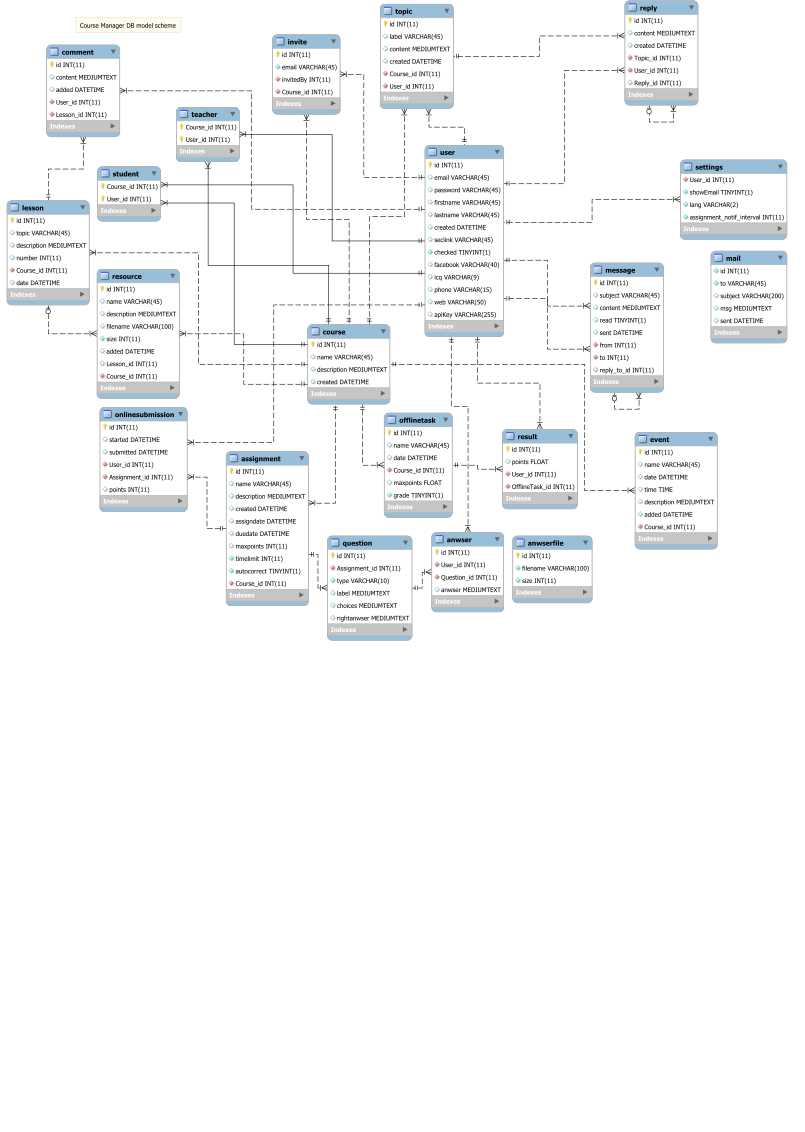
\includegraphics[scale=0.35]{\lyxdot \lyxdot /db/scheme}

\caption{Schéma databázového modelu webové aplikace. Vygenerováno programem
\emph{MySQL Workbench}.}


\end{sidewaysfigure}
\label{chap:schemadb}

\settowidth{\nomlabelwidth}{MySQL}
\printnomenclature{}

\newpage{}\bibliographystyle{plain}
\phantomsection\addcontentsline{toc}{chapter}{\bibname}\nocite{*}
\bibliography{bib}

\end{document}
